%%
%% Anexos.tex
%% Projeto Oficinas de Integração 3
%% Created by Leonardo Winter Pereira and Lucas Zimmermann Cordeiro on 10.03.2016
%% Copyright (C). All rights reserved
%%

%% Anexo é um texto ou documento não elaborado pelo autor
%% do Trabalho Científico (TC) (monografia, tese, etc.)

\chapter{Datasheets}
\label{chap:anexosA}

    Este capítulo compreende todos os \textit{datasheets} de terceiros utilizados durante o desenvolver do projeto.

    É importante ressaltar que os componentes desenvolvidos pela própria equipe, sistemas eletrônicos e códigos estão todos relatados no capítulo anterior.

    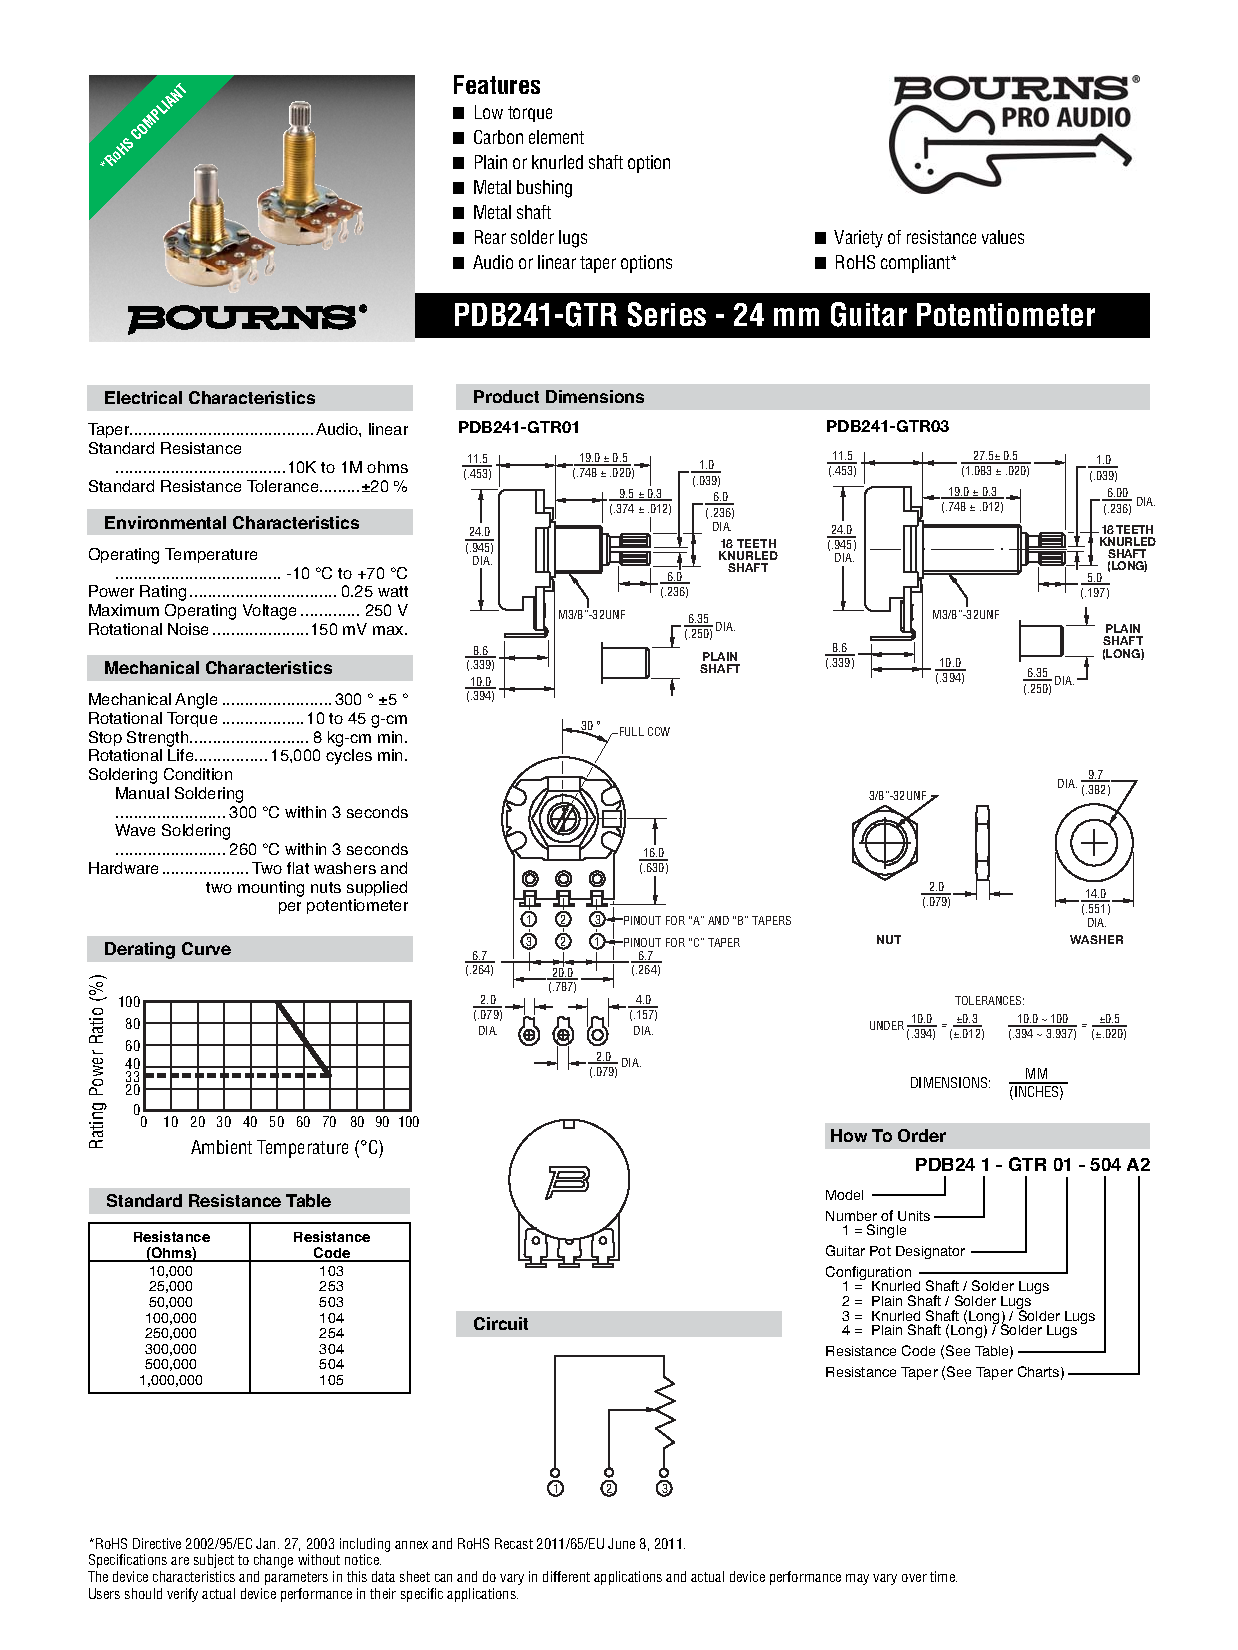
\includepdf[scale={0.8}, pages={1}, pagecommand=\section{Potenciômetro rotativo}]{../Datasheets/rotary_potentiometer.pdf}

    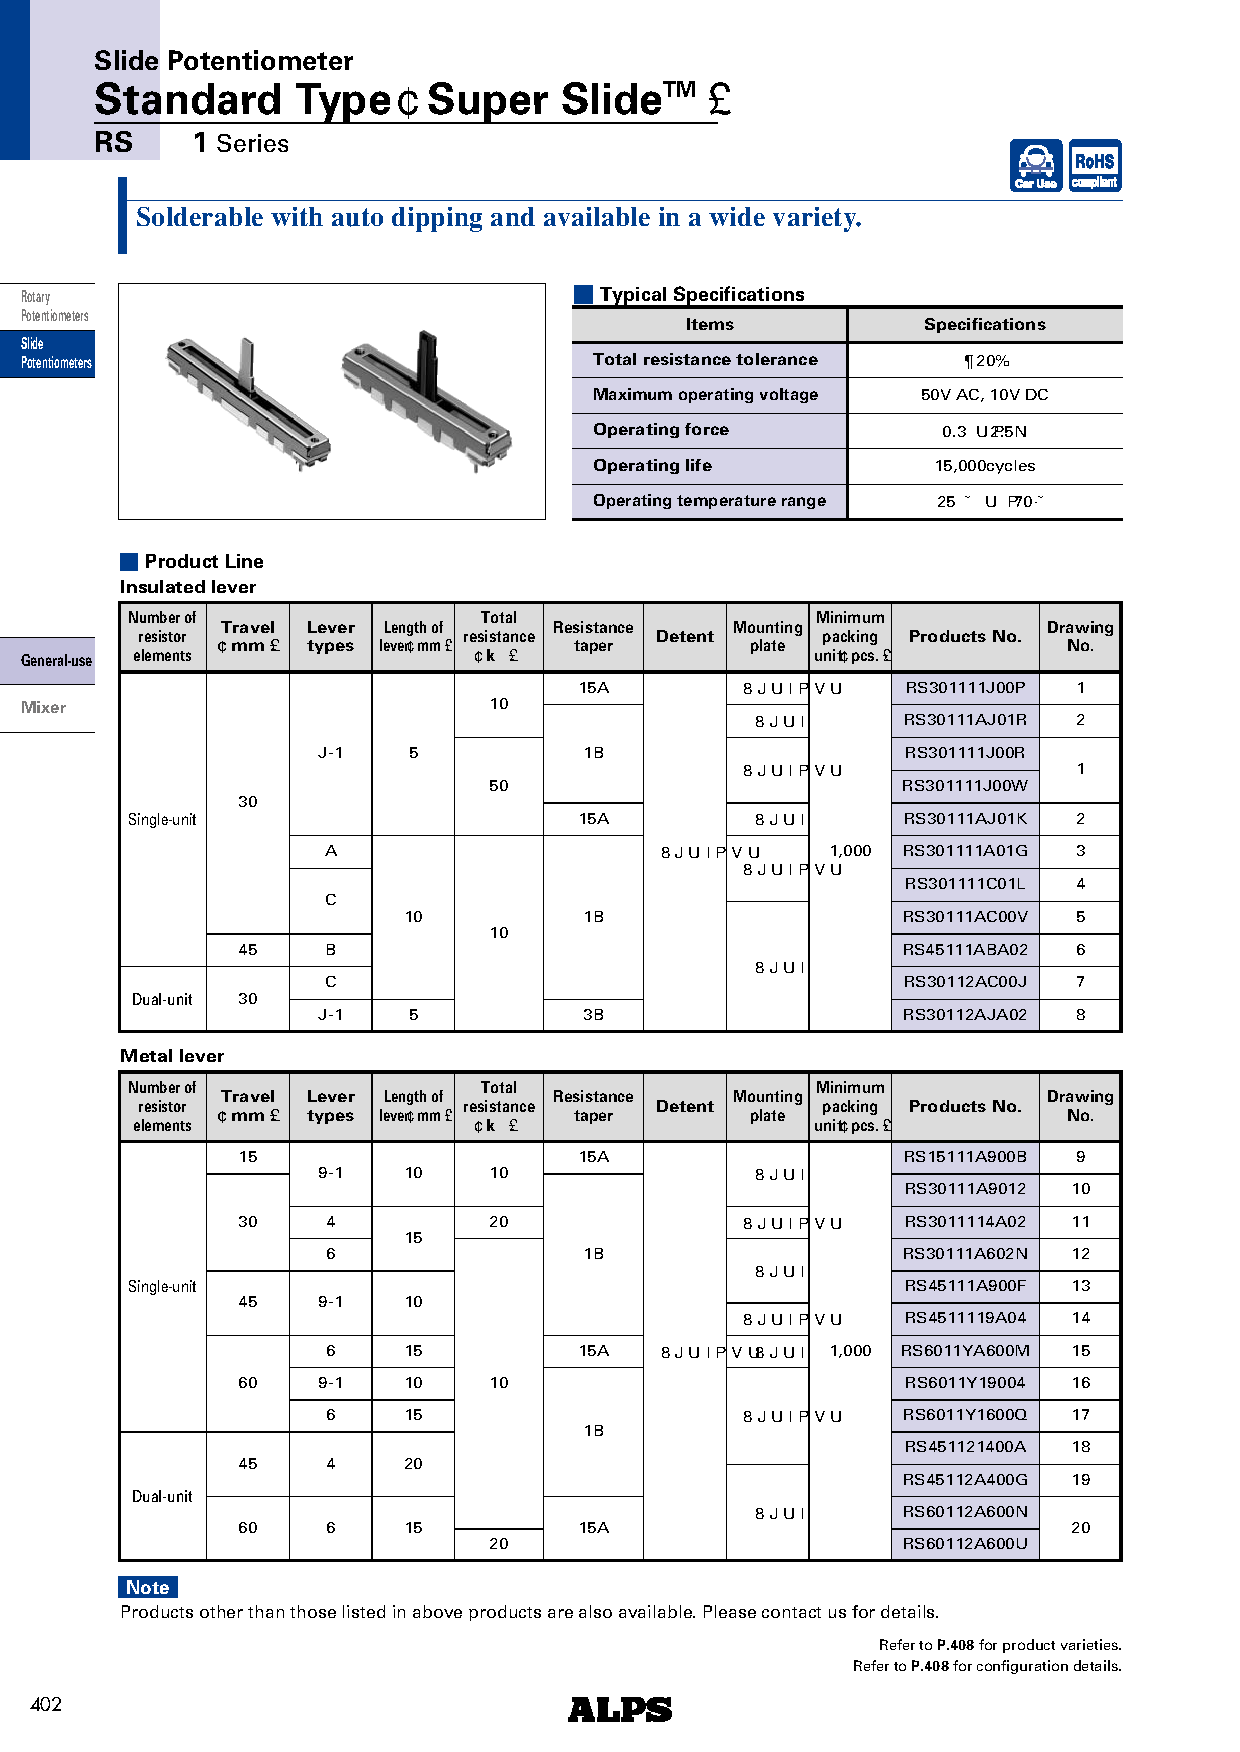
\includepdf[scale={0.7}, pages={1}, pagecommand=\section{Potenciômetro linear}]{../Datasheets/linear_potentiometer_b10k.pdf}
    \includepdf[scale={0.8}, pages={6}, pagecommand={}]{../Datasheets/linear_potentiometer_b10k.pdf}
    \includepdf[scale={0.8}, pages={9}, pagecommand={}]{../Datasheets/linear_potentiometer_b10k.pdf} 